\begin {document}

\title {\ZHH \huge 学习ejoy2d——spritepack}
\author {\small gaccob}
\date {\small 2014 年 3 月 12 日}
\maketitle

{在学习sprite之前, 先了解一下sprite\_pack, lib/sprite\_pack.h和lib/sprite\_pack.c提供了底层的数据操作. ejoy2d/spritpack.lua封装了上层接口, 提供数据之间的打解包转换.}\par

\begin {figure}[htbp]
    \centering
    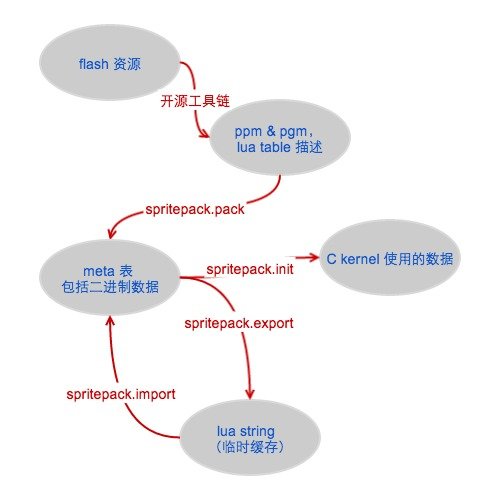
\includegraphics [width=350pt, keepaspectratio] {sprite_pack.jpg}
\end {figure}

{"这只是方便开发,在产品发行时不应该这样做". 从版本的安全性来说, 还需要做一些加密工作, 防止资源被破解. }\par

{关于资源, 根据github文档所述, 有\href{https://github.com/robinxb/flash-parser}{开源工具}支持从 cocos builder 中导出. }\par

{sprite目前支持5种图元:}\par
\begin{lstlisting}[language=C]
#define TYPE_EMPTY 0
#define TYPE_PICTURE 1
#define TYPE_ANIMATION 2
#define TYPE_POLYGON 3
#define TYPE_LABEL 4
#define TYPE_PANNEL 5
// `\color{gray} anchor是一个比较特殊的类型, 它没有资源数据, 仅提供了一个锚点, 可以挂载其他sprite`
#define TYPE_ANCHOR 6

// `\color{gray} TYPE\_PICTURE 四边形`
struct pack_picture {
    int n;
    struct pack_quad rect[1];
};

// `\color{gray} TYPE\_ANIMATION 动画`
struct pack_animation {
    int frame_number;
    int action_number;
    int component_number;
    struct pack_frame *frame;
    struct pack_action *action;
    struct pack_component component[1];
};

// `\color{gray} TYPE\_POLYGON 多边形`
struct pack_poly {
    int texid;
    int n;
    uint16_t *texture_coord;
    int32_t *screen_coord;
};

// `\color{gray} TYPE\_LABEL 文字框`
struct pack_label {
    uint32_t color;
    int width;
    int height;
    int align;
    int size;
    int edge;
    int max_width;
};

// `\color{gray} TYPE\_PANNEL 面板`
struct pack_pannel {
    int width;
    int height;
    int scissor;
};

// `\color{gray} component可以是任意sprite, 但是要自己保证不能成环`
struct pack_component {
    int id;
    const char *name;
};

// `\color{gray} 这就是导入的lua描述文件的C数据结构`
// `\color{gray} data数组的下标是sprite的id, 也就是component引用的id.`
struct sprite_pack {
    int n;
    uint8_t * type;
    void ** data;
    int tex[1];
};
\end{lstlisting}

{spritepack的C代码中最重要的就是limport()函数, 它负责导入二进制资源.}\par
\begin{lstlisting}[language=C]
// `\color{gray} lua的输入参数格式:`
// `\color{gray}    number: texture id |  table: texture id table`
// `\color{gray}    number: max id, pack对象的最大id`
// `\color{gray}    number: max userdata size, 分配器的buffer size`
// `\color{gray}    string: data | lightuserdate: data`
//              `\color{gray}    | number: data size`
static int
limport(lua_State *L) {
    ...

    // `\color{gray} 一个简单的内存分配器, 保证了内存都from Lua (userdata)`
    struct import_alloc alloc;
    alloc.L = L;
    alloc.buffer = (char *)lua_newuserdata(L, size);
    alloc.cap = size;
   
    // `\color{gray} 分配sprite\_pack, 并初始化`
    struct sprite_pack *pack = (struct sprite_pack *)ialloc(&alloc, sizeof(*pack) + (tex - 1) * sizeof(int));
    pack->n = max_id + 1;

    // `\color{gray} 分配type, 4字节对齐(type是uint8)`
    int align_n = (pack->n + 3) & ~3;
    pack->type = (uint8_t *)ialloc(&alloc, align_n * sizeof(uint8_t));
    memset(pack->type, 0, align_n * sizeof(uint8_t));
    
    // `\color{gray} 分配data指针`
    pack->data = (void **)ialloc(&alloc, pack->n * sizeof(void*));
    memset(pack->data, 0, pack->n * sizeof(void*));

    // `\color{gray} 导入texure id`
    if (lua_istable(L,1)) {
        int i;
        for (i=0; i<tex; i++) {
            lua_rawgeti(L,1,i+1);
            pack->tex[i] = (int)luaL_checkinteger(L, -1);
            lua_pop(L,1);
        }
    } else {
        pack->tex[0] = (int)lua_tointeger(L,1);
    }

    // `\color{gray} 构造一个输入数据流(指向目标资源数据), 方便后续导入`
    struct import_stream is;
    is.alloc = &alloc;
    is.pack = pack;
    is.current_id = -1;
    if (lua_isstring(L,4)) {
        is.stream = lua_tolstring(L, 4, &is.size);
    } else {
        is.stream = (const char *)lua_touserdata(L, 4);
        if (is.stream == NULL) {
            return luaL_error(L, "Need const char *");
        }
        is.size = luaL_checkinteger(L, 5);
    }

    // `\color{gray} 依次从数据流中导入数据`
    while (is.size != 0) {
        import_sprite(&is);
    }

    return 1;
}
\end{lstlisting}

{需要注意的是, sprite\_pack数据内存(包括了它的所有图元), 都是从分配器(源自Lua)中分配, "C对象生命周期全部由Lua VM管理". }\par

{spritepack.lua的接口pack()和init(), 将 lua table 资源打包成元数据, 或者在运行时从元数据中导入二进制数据. 结合example里的sample.lua范例, 很好理解.}\par

\begin{lstlisting}[language=lua]

-- `\color{gray} 输入的data是lua table, 参照example/sample.lua`
-- `\color{gray} 返回值是meta表`
function spritepack.pack(data)
    local ret = { texture = 0, maxid = 0, size = 0 , data = {}, export = {} }
    local ani_maxid = 0

    for _,v in ipairs(data) do
        if v.type ~= "particle" then

            -- `\color{gray} 唯一id`
            local id = assert(tonumber(v.id))
            if id > ret.maxid then
                ret.maxid = id
            end

            -- `\color{gray} export name 不是必须的, sample里只有两个animation有`
            local exportname = v.export
            if exportname then
                assert(ret.export[exportname] == nil, "Duplicate export name"..exportname)
                ret.export[exportname] = id
            end

            table.insert(ret.data, pack.word(id))

            -- `\color{gray} 根据type分别pack`
            if v.type == "picture" then
                local sz, texid = pack_picture(v, ret.data)
                ret.size = ret.size + sz
                if texid > ret.texture then
                    ret.texture = texid
                end
            elseif v.type == "animation" then
                local sz , maxid = pack_animation(v, ret.data)
                ret.size = ret.size + sz
                if maxid > ani_maxid then
                    ani_maxid = maxid
                end
            elseif v.type == "polygon" then
                local sz, texid = pack_polygon(v, ret.data)
                ret.size = ret.size + sz
                if texid > ret.texture then
                    ret.texture = texid
                end
            elseif v.type == "label" then
                local sz = pack_label(v, ret.data)
                ret.size = ret.size + sz
            elseif v.type == "pannel" then
                local sz = pack_pannel(v, ret.data)
                ret.size = ret.size + sz
            else
                error ("Unknown type " .. tostring(v.type))
            end
        end
    end

    if ani_maxid > ret.maxid then
        error ("Invalid id in animation ".. ani_maxid)
    end

    ret.texture = ret.texture + 1

    -- `\color{gray} 这里把table做了一次拼接`
    ret.data = table.concat(ret.data)

    ret.size = ret.size + pack.pack_size(ret.maxid, ret.texture)
    return ret
end

function spritepack.init( name, texture, meta )
    assert(pack_pool[name] == nil , string.format("sprite package [%s] is exist", name))
    if type(texture) == "number" then
        assert(meta.texture == 1)
    else
        assert(meta.texture == #texture)
    end
    
    -- `\color{gray} 调用C接口来实现载入资源`
    pack_pool[name] = {
        cobj = pack.import(texture,meta.maxid,meta.size,meta.data, meta.data_sz),
        export = meta.export,
    }
    meta.data = nil

    return pack_pool[name]
end
\end{lstlisting}

{spritepack.lua的接口export()和import(), 对pack后的meta数据做打包成字符串, 或者从字符串解包.}\par
{github上文档原文: "可以用 spritepack.export 在开发期预处理 spritepack.pack 生成的结果, spritepack.export 返回一个字符串,可将这个字符串持久化到文件中". } \par

\begin{lstlisting}[language=lua]
function spritepack.export(meta)
    local result = { true }
    table.insert(result, pack.word(meta.maxid))
    table.insert(result, pack.word(meta.texture))
    table.insert(result, pack.int32(meta.size))
    table.insert(result, pack.int32(#meta.data))
    local s = 0
    for k,v in pairs(meta.export) do
        table.insert(result, pack.word(v))
        table.insert(result, pack.string(k))
        s = s + 1
    end
    result[1] = pack.word(s)
    table.insert(result, meta.data)
    return table.concat(result)
end

function spritepack.import(data)
    local meta = { export = {} }
    local export_n, off = pack.import_value(data, 1, 'w')
    meta.maxid , off = pack.import_value(data, off, 'w')
    meta.texture , off = pack.import_value(data, off, 'w')
    meta.size , off = pack.import_value(data, off, 'i')
    meta.data_sz , off = pack.import_value(data, off, 'i')
    for i=1, export_n do
        local id, name
        id, off = pack.import_value(data, off, 'w')
        name, off = pack.import_value(data, off, 's')
        meta.export[name] = id
    end
    meta.data = pack.import_value(data, off, 'p')

    return meta
end
\end{lstlisting}

\end{document}

